\chapter{FreeRTOS Implementation}
\label{cha:rtos}

\textit{STEERED} has been developed and tested on bare-metal applications to ensure
its correctness in simple environments. However, many embedded devices are designed
to accomplish more complex tasks and they need special environments to support the
execution. In this section, we provide a description on how \textit{Free Real
Time Operating System} (\textit{FreeRTOS}) could be implemented together with \textit{STEERED}
to secure and support complex tasks.

\section{FreeRTOS}
\label{sec:rtos_rtos}

\textit{FreeRTOS}\cite{freertos} is an open-source, lightweight, Real-Time Operating
System (\textit{RTOS}) kernel designed for embedded systems. In recent years,
\textit{FreeRTOS} has become one of the most widely used \textit{RTOS} kernels
in embedded applications, particularly in microcontrollers, because of its
simplicity, efficiency, scalability, and portability.

\textit{FreeRTOS} is mostly used in applications that require reliable, deterministic
behavior in resource-constrained environments. Some examples are: medical devices,
IoT devices, automotive and many more.

\subsection{FreeRTOS Features}
\label{subsec:rtos_features}

\textit{FreeRTOS} provides many features, the most important being:
\begin{itemize}
  \item Real-Time Scheduling: \textit{FreeRTOS} supports real-time scheduling with
    both preemptive and cooperative multitasking. In preemptive scheduling, tasks
    are prioritized and can interrupt lower-priority tasks, while in cooperative
    multitasking, tasks yield control to others explicitly. Moreover, it uses a priority-based
    scheduling, allowing developers to assign priority levels to tasks based on
    their timing requirements;

  \item Task Management: Tasks in \textit{FreeRTOS} are individual threads of execution,
    each with its own stack and context. The kernel allows the creation,
    deletion, and management of tasks dynamically. Each task operates in its own
    context, which the kernel saves and restores during context switching;

  \item Memory Management: \textit{FreeRTOS} provides several memory allocation schemes,
    including static and dynamic allocation, through its portable memory allocation
    subsystem. It supports different heap management schemes (\textit{heap\_1}
    through \textit{heap\_5}), offering varying levels of complexity and memory usage
    optimization. These schemes allow developers to balance between simplicity
    and flexibility;

  \item Interrupt Handling: \textit{FreeRTOS} is designed to work seamlessly with
    hardware interrupts, allowing Interrupt Service Routines (ISR) to
    communicate with tasks through mechanisms like queues and semaphores. The kernel
    offers a low-latency method for ISR handling, enabling efficient
    communication between ISRs and tasks while ensuring minimal delay in task
    scheduling;

  \item Software Timers: \textit{FreeRTOS} includes a timer API, allowing
    developers to create software timers that automatically trigger callback
    functions after a specified period. This feature helps to manage time-dependent
    operations without creating dedicated tasks;

  \item Portability and Scalability: \textit{FreeRTOS} is highly portable and can
    be adapted to run on numerous processor architectures, including \textit{ARM
    Cortex-M}, \textit{ARM Cortex-A}, \textit{RISC-V}, and various other
    architectures. It is structured in a way that allows developers to scale applications
    easily by adding or removing tasks, memory management schemes, and communication
    mechanisms as needed;

  \item Debugging and Traceability: \textit{FreeRTOS} provides support for debugging
    and traceability, offering hooks that allow users to gather runtime
    statistics and monitor task execution patterns.
\end{itemize}

With all these features it is easy to see why \textit{FreeRTOS} has become a standard
in the community. However, \textit{FreeRTOS} presents some limitations like the
limited built-in security and the lack of support for multicore processing. Some
of this flaws have been addressed by community users and companies with alternative
versions of the Operating System. For example, \textit{Espressif} presented
\textit{IDF FreeRTOS}\cite{idfrtos}, a version of \textit{FreeRTOS} which
provides support for multicore processing. Moreover, \textit{highintegritysystems}
developed \textit{SAFERTOS}\cite{safertos}, a redesign of the \textit{FreeRTOS} kernel
to enhance security.

Overall, \textit{FreeRTOS} is a powerful choice for developers working with embedded
systems that require real-time capabilities, low overhead, and efficient resource
management. Its design balances simplicity with flexibility, making it suitable for
a wide variety of applications from small IoT devices to more complex industrial
systems.

\section{FreeRTOS and STEERED}
\label{sec:rtos_porting}

In this section, we provide a detailed description on how \textit{FreeRTOS}
could be imported inside \textit{STEERED} and why this could increase the scenarios
in which \textit{STEERED} could be used.

We have seen that \textit{STEERED} is designed to securely run untrusted user-code
in bare-metal environments. However, given its simplicity it could be used to secure
code in more complex environments, for example with a Real Time Operating System
like \textit{FreeRTOS}.

The main idea is to maintain \textit{STEERED} as the M-mode operator, managing system
boot and edge controls. The user code in this case is represented by the various
tasks generated thanks to \textit{FreeRTOS}. Code instrumentation would not
change much as we would just need to add the \textit{regex} functions to search for
\textit{FreeRTOS}-specific instructions that cause a control transfer during
execution. Finally, \textit{FreeRTOS} could be used as a ``supervisor'', either
trusted or untrusted depending on the case. It would be in charge of managing task
scheduling and memory operations.

Moreover, since \textit{FreeRTOS} requires its own Interrupt Service Routine we could
either:
\begin{itemize}
  \item Prepare two separate Interrupt Vector Tables, one for \textit{STEERED}\footnote{The
    same we have seen in Section \ref{sec:project_isr}} and one for \textit{FreeRTOS}.
    However, traps at user level are managed by default ad machine level so, if
    we have an interrupt or an exception in one of the tasks the controls is
    transferred to the \textit{STEERED} interrupt vector table and we must manually
    transfer the flow to the correct handler of the \textit{FreeRTOS} interrupt
    vector table;

  \item Another solution could be to prepare two separate interrupt vector tables
    and use \textit{mideleg} and \textit{medeleg} registers (seen in Section
    \ref{subsec:riscv_deleg}) to automatically delegate some interrupts and/or exceptions
    to the \textit{FreeRTOS} interrupt vector table. For example, if we know
    that user interrupts are always managed by \textit{FreeRTOS} we could insert
    the corresponding code inside \textit{mideleg}. With this, each time a user-level
    interrupt is generated it is trapped at the \textit{FreeRTOS} interrupt vector
    table. Note that this does not mean that \textit{STEERED} will not be able to
    manage those traps as higher level interrupts and exception can't be delegated
    to lower level handler. For example, if a machine-level interrupt is generated
    it will always be handled by \textit{STEERED} interrupt vector table.
\end{itemize}

\section{Porting Limitations}
\label{sec:rtos_limitations}

The presented implementation present one key limitation, \textit{FreeRTOS} needs
to perform some operations on Control and Status Registers to function correctly
but, as we have explained such registers are only available in machine mode.
Since the implementation inside \textit{STEERED} would require \textit{FreeRTOS}
to run either in supervisor or user mode all those operations would generate an
illegal instruction exception as those privilege modes can't access machine CSRs.
Some of these operations are depicted in Listing \ref{lst:freeoperations}.

To address this problem we could enhance the instrumentation phase to modify \textit{FreeRTOS}'s
code in the following way. Firstly, we need to find the critical instructions, this
can be done easily with \textit{regex} functions. With this we can extract the operation
that \textit{FreeRTOS} is trying to perform (among the one seen in Section \ref{sec:riscv_csrs})
and the target CSR. The target CSR can be then translated thanks to the table \textit{Currently
allocated RISC-V machine-level CSR addresses}\footnote{Provided by the \textit{RISC-V
Privileged Manual}\cite{riscv} at page $17$.} where we can see that for example register
\textit{mstatus} is referred to as number $0x300$. Now we can precisely describe
each target CSR and we just need to inject new instructions to perform an \textit{ECALL}
to \textit{STEERED}'s interrupt vector table which will perform the modification
of the CSRs on behalf of \textit{FreeRTOS}.

\begin{lstlisting}[style=Assembly, caption = \textit{FreeRTOS} operations on Control and Status Registers, label={lst:freeoperations}]
  csrr a0, mcause  // Store inside register a0 the value of mcause
  csrw mepc, a0    // Write mepc with the value of a0
  csrs mstatus, t0 // Set bit(s) in mstatus based on value of t0
  csrc mie, a0     // Clear bit(s) in mie based on value of a0
  \end{lstlisting}

To do so, we can choose between two options. The first is to use register \textit{a7}
to hold the new \textit{ECALL} code which determines the operation and two other
registers, say \textit{a6} and \textit{a5} to hold the CSR number and the CSR
instruction respectively. However, this solution is highly inefficient in the
use of registers since we could encode those values into $2$ registers instead
of $3$. Alternatively, we could use register \textit{a7} to hold the new \textit{ECALL}
code and \textit{a6} to hold the CSR number and the CSR instruction. Since there
are $3$ CSR instructions we just need $2$ bits to encode them, Table \ref{tab:instructionenc}
depicts a possible representation of the encodings of CSR instructions. All
other bits would be reserved to describe the target CSR for the operation. Note that
CSRs numbers go from $0x300$ up to $0xf15$ so we need at maximum $12$ bits to represent
each of them. Also, we can't encode the \textit{ECALL} code inside the same
register because we are using the least significant bit to represent forward and
backward edge controls thus, using it would result in ambiguity on the operation
to perform.

\begin{table}
  \centering
  \begin{tabular}{|c|c|c|}
    \hline
    \textbf{Number} & \textbf{Value} & \textbf{Instruction} \\
    \hhline{===} 1  & $00$           & CSRRW                \\
    \hline
    2               & $01$           & CSRRS                \\
    \hline
    3               & $10$           & CSRRC                \\
    \hline
    4               & $11$           & Reserved             \\
    \hline
  \end{tabular}
  \caption{CSR instructions encoding}
  \label{tab:instructionenc}
\end{table}

Figure \ref{fig:a6encoding} a depicts a possible encoding for register \textit{a6}
where we use the two most significant bits to encode the CSR instruction we want
to perform and all the other bits to represent the target CSR.

\begin{figure}[htbp]
  \centering
  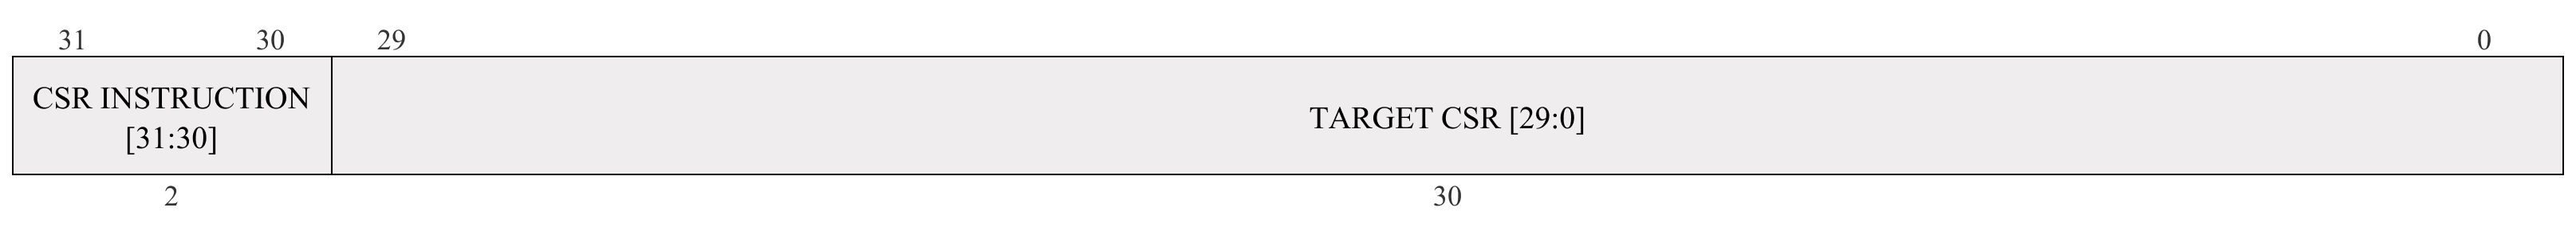
\includegraphics[width=.9\linewidth]{images/freertos_encoding.png}
  \caption{Possible encoding for register \textit{a6}}
  \label{fig:a6encoding}
\end{figure}

Lastly, we would just need to add an if statement inside \textit{STEERED}'s
interrupt vector table to determine if we are requesting to perform a CSR
instruction on behalf of \textit{FreeRTOS}.

Note that this is just a proposal of implementation and there may be other ways to
implement \textit{FreeRTOS} inside \textit{STEERED}.